%%%%%%%%%%%%%%%%%%%%%%%%%%%%%%%%%%%%%%%%%
% Beamer Presentation
% LaTeX Template
% Version 1.0 (10/11/12)
%
% This template has been downloaded from:
% http://www.LaTeXTemplates.com
%
% License:
% CC BY-NC-SA 3.0 (http://creativecommons.org/licenses/by-nc-sa/3.0/)
%
%%%%%%%%%%%%%%%%%%%%%%%%%%%%%%%%%%%%%%%%%

%----------------------------------------------------------------------------------------
%	PACKAGES AND THEMES
%----------------------------------------------------------------------------------------

\documentclass{beamer}

\mode<presentation> {

% The Beamer class comes with a number of default slide themes
% which change the colors and layouts of slides. Below this is a list
% of all the themes, uncomment each in turn to see what they look like.

%\usetheme{default}
%\usetheme{AnnArbor}
%\usetheme{Antibes}
%\usetheme{Bergen}
%\usetheme{Berkeley}
\usetheme{Berlin}
%\usetheme{Boadilla}
%\usetheme{CambridgeUS}
%\usetheme{Copenhagen}
%\usetheme{Darmstadt}
%\usetheme{Dresden}
%\usetheme{Frankfurt}
%\usetheme{Goettingen}
%\usetheme{Hannover}
%\usetheme{Ilmenau}
%\usetheme{JuanLesPins}
%\usetheme{Luebeck}
%\usetheme{Madrid}
%\usetheme{Malmoe}
%\usetheme{Marburg}
%\usetheme{Montpellier}
%\usetheme{PaloAlto}
%\usetheme{Pittsburgh}
%\usetheme{Rochester}
%\usetheme{Singapore}
%\usetheme{Szeged}
%\usetheme{Warsaw}

% As well as themes, the Beamer class has a number of color themes
% for any slide theme. Uncomment each of these in turn to see how it
% changes the colors of your current slide theme.

%\usecolortheme{albatross}
%\usecolortheme{beaver}
%\usecolortheme{beetle}
%\usecolortheme{crane}
%\usecolortheme{dolphin}
%\usecolortheme{dove}
%\usecolortheme{fly}
%\usecolortheme{lily}
%\usecolortheme{orchid}
%\usecolortheme{rose}
%\usecolortheme{seagull}
%\usecolortheme{seahorse}
%\usecolortheme{whale}
%\usecolortheme{wolverine}

%\setbeamertemplate{footline} % To remove the footer line in all slides uncomment this line
%\setbeamertemplate{footline}[page number] % To replace the footer line in all slides with a simple slide count uncomment this line

%\setbeamertemplate{navigation symbols}{} % To remove the navigation symbols from the bottom of all slides uncomment this line
}
\usepackage{color}
\newenvironment{variableblock}[3]{%
  \setbeamercolor{block body}{#2}
  \setbeamercolor{block title}{#3}
  \begin{block}{#1}}{\end{block}}
\usepackage{graphicx} % Allows including images
\usepackage{booktabs} % Allows the use of \toprule, \midrule and \bottomrule in tables

%----------------------------------------------------------------------------------------
%	TITLE PAGE
%----------------------------------------------------------------------------------------

\title[]{Lab 7 Presentation} % The short title appears at the bottom of every slide, the full title is only on the title page

\author{Anand Chandrakant Pisal} % Your name
\institute[IIT Bombay] % Your institution as it will appear on the bottom of every slide, may be shorthand to save space
{
IIT Bombay \\ % Your institution for the title page
\medskip
\textit{183059001@iitb.ac.in} % Your email address
}
\date{\today} % Date, can be changed to a custom date


\setbeamertemplate{headline}
 {%
  \begin{beamercolorbox}[ht=2.5ex,dp=1.125ex]{section in head/foot}
  \insertsectionnavigationhorizontal{\textwidth}{}{}
  \end{beamercolorbox}%
   \begin{beamercolorbox}[ht=2.5ex,dp=1.125ex]{subsection in head/foot}
   \end{beamercolorbox}%
}


\begin{document}
\begin{frame}
\titlepage
\end{frame}
\begin{frame}{Topics to cover}
	\tableofcontents
\end{frame}
\section{Important Theorem}
\begin{frame}{Important Theorem}
\begin{columns}
\begin{column}[T]{\textwidth}
  	\begin{block}<1->{Newton Second law \footnote[frame]{This is the standard way of reference}}
    Acceleration of a body is directly proportional to the force applied
on it and inversely proportional to the mass of the body. This
theorem derives the equation
	\center {\emph{F = ma}}
	\vspace{0.5cm}
  	\end{block}
  	 \setbeamercolor{block title}{fg=black,bg=green!60!black}
    \setbeamercolor{block body}{fg=black,bg=green!10}
  	\begin{theorem}<2->[Pythagorean theorem]
    \center{h\textsuperscript{2} = b\textsuperscript{2} + p\textsuperscript{2}}
    \vspace{0.5cm}
  	\end{theorem}
\end{column}
\end{columns}	
\end{frame}

\section{Match Result}
\begin{frame}{Cricket Result}
\begin{columns}
\begin{column}[T]{0.3\textwidth}
\vspace{0.5cm}
\textbf {Team 1}
\begin{enumerate}
  \item India
  \item Pakistan
  \item Bangladesh
\end{enumerate}
\end{column}
\begin{column}[T]{0.3\textwidth}
\vspace{0.5cm}
\textbf {Team 2}
\begin{enumerate}
  \item Australia
  \item South Africa
  \item West Indies
\end{enumerate}
\end{column}
\begin{column}[T]{0.3\textwidth}
\textbf {Result}
\begin{enumerate}
  \item Indai won
  \item South Africa won
  \item Bangladesh won
\end{enumerate}
\end{column}
\end{columns}	




\end{frame}

\section{My Expenses}
\begin{frame}{Semester expenses}
\begin{figure}
\centering
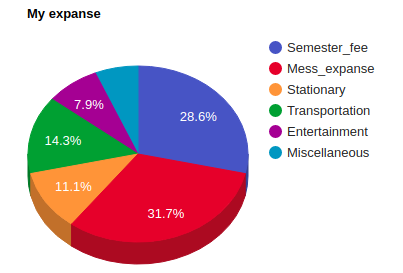
\includegraphics[scale=0.5]{pie_chart.png}
\end{figure}
\end{frame}

\section{Important Formula}
\begin{frame}{XOR Gate}
\begin{table}[h!]
  \begin{center}
    \begin{tabular}{p{1cm} p{1cm} p{1cm}}
      \hline
	  \textbf{X} & \textbf{Y} & \textbf{Z}\\
      \hline
      TRUE & TRUE & FALSE\\
      TRUE & FALSE & TRUE\\
      FALSE & TRUE & TRUE\\
      FALSE & FALSE & FALSE\\
      \hline
    \end{tabular}
    \caption{Truth Table}
  \end{center}
\end{table}
\end{frame}

\begin{frame}
\center
{\begin{Huge}
The End
\end{Huge}}
\end{frame}

\end{document}\grid
\grid
